% \parencite[see][]{einstein}
%\cite{latexcompanion}

%\begin{figure}[h]
%    \centering
%	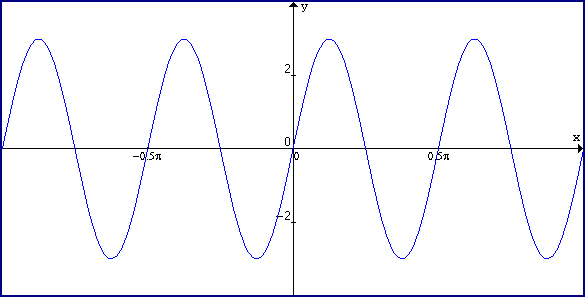
\includegraphics[scale=0.5]{graph}
%	\caption{An example graph}
%	\label{fig:x sine graph}
%\end{figure}

The core of this algorithm is take from \cite{event-detection}.

\section{Document fetching}
We assume a collection of documents $\{d_{1}, d_{2}, \dots, d_{D}\}$ where for each document $d_{i}$, we know its publication day $t_{i}$. Then, the documents can be understood as a stream $\{(d_{1}, t_{1}), (d_{2}, t_{2}), \dots, (d_{D}, t_{D})\}$ with $t_{i} \leq t_{j}$ for $i < j$. Furthermore, we define $T$ to be the length of the stream, and we normalize the document publication days to be relative to the document stream start; that is $t_{1} = 0$ and $t_{D} = T - 1$.


\section{Bag of words model}
% TODO: blah blah we use the well known (binary) bag of words model, which drops the word order
To vectorize the documents, we define a matrix $\mathbf{B} \in \{0, 1\}^{D \times V}$ where V is the total vocabulary size. The document collection can then be understood as a set of $D$ observations, each consisting of $V$ binary features. The matrix $\mathbf{B}$ is defined as

\begin{equation}
	\mathbf{B}_{ij} = \begin{cases}
		1, & \text{document}~i~\text{contains the feature}~j \text{;} \\
		0, & \text{otherwise.}
	\end{cases}
\end{equation}

To limit the feature space, we trim the words appearing in less than 30 documents or in more than 90\% of the documents. The idea behind this is that the words appearing only in few documents cannot possibly represent relevant events, and are mostly anomalies. On the other hand, words appearing in most of the documents are likely stopwords, and do not carry much information.

From now on, we focus our analysis on the individual word features rather than whole documents.

\section{Computing feature trajectories}
The previous section represented word features in the document domain. This section focuses on representing these features in the time domain.

A time trajectory of a feature $f$ is a vector $\mathbf{y}_f = \big(y_{f}(1), y_{f}(2), \dots, y_{f}(T)\big)$. Each element $y_{f}(t)$ represents the relative frequency of the feature $f$ at time $t$. This frequency is defined using the DFIDF score:

\begin{equation}
	y_{f}(t) \coloneqq \frac{\text{DF}_{f}(t)}{\text{D}(t)} \times \log{\frac{\text{D}}{\text{DF}_{f}}},
\end{equation}

where $\text{DF}_{f}(t)$ is the number of documents published on day $t$ which contain the feature $f$ (time-local document frequency), $\text{D}(t)$ is the number of documents published on day $t$ and $\text{DF}_{f}$ is the number of documents containing the feature $f$ (global document frequency).

These feature trajectories are stored in a matrix $\mathbf{T} \in \R^{V \times T}$, with $\mathbf{y}_f$ being the $f$-th row of $\mathbf{T}$.


\section{Spectral analysis}
The next step is to employ spectral analysis techniques borrowed from signal processing to discover periodicities in the features. Results from this section are used in the next section to categorize word features.

The well known discrete Fourier transform is applied to each feature trajectory, yielding $\mathcal{F} \mathbf{y}_y = \big(X_{1}, X_{2}, \dots, X_{T}\big)$ such that

\begin{equation}
	X_{k} = \sum_{t = 1}^{T}{y_{f}(t) \me^{- \frac{2 \pi \mi}{T} (k - 1) t}}, ~ k \in \{1, 2, \dots, T\}.
\end{equation}

The periodogram estimator is then used to estimate the power spectral density from the Fourier coefficients $X_{k}$.
% TODO: Write about periodogram.

We define the dominant power spectrum of the feature $f$ as

\begin{equation}
	\text{DPS}_{f} \coloneqq \max_{k \leq \ceil{T/2}}{\|X_{k}\|^{2}},
\end{equation}

and the dominant period as

\begin{equation}
	\text{DP}_{f} \coloneqq \frac{1}{\mathit{freq}}.
\end{equation}

where \textit{freq} is the frequency corresponding to $\text{DPS}_{f}$.


\section{Feature categorization}
Based on the dominant power spectra and dominant periods, we divide the features into two categories \footnote{\cite{event-detection} actually define \textit{five} such categories; however, our method uses only two of them.}:

\begin{equation}
	\mathit{HH} \coloneqq \{f \mid DPS(f) > \textit{dps-bound}, ~ DP(f) > \ceil{T / 2}\},
\end{equation}

\begin{equation}
	\mathit{HL} \coloneqq \{f \mid DPS(f) > \textit{dps-bound}, ~ DP(f) \leq \ceil{T / 2}\},
\end{equation}

The \textit{HH} category corresponds to High power-High period features. Similarly, the \textit{HL} category corresponds to High power-Low period features.

% TODO: Create a pretty figure.


\section{Event detection}

\subsection{Measuring trajectory similarity}

\subsection{Measuring document overlap}

\subsection{Event detection}